Scientific applications and workflows use a diverse set of tools to execute 
tasks on HPC resources with diverse requirements and performance. Simulations 
are mainly parallelized through MPI. On the other hand, several parallel 
frameworks and techniques, such as MPI, Spark~\cite{zaharia2010spark}, 
Hadoop~\cite{hadoop}, and Dask~\cite{rocklin2015dask}, are being used to 
execute data analytics in addition to machine and deep learning techniques. 
Executing complex workflows that produce and analyze data requires to support 
MPI style execution along with data-parallel techniques. As a result, extended 
a task parallel workload execution framework on HPC to support, in addition to 
MPI, data parallel frameworks. Furthermore, we investigated the suitability of 
different data and task parallel frameworks for different types of analysis.

\subsection{Providing Data-Parallel capabilities on HPC}
Managing high performance and data intensive application stages on HPC resources 
is necessary. The pilot abstraction~\cite{turilli2018comprehensive}, via its 
implementation RADICAL-Pilot~\cite{merzky2019using}, has successfully used to 
parallelize task level execution of scientific simulations on HPC resources. 
Thus, we extended RADICAL-Pilot to support data intensive applications on HPC 
resources. 


\subsection{Conceptual Model for Task-Parallel framework selections}
Task-parallel applications involve partitioning a workload into a set of self-
contained units of work. Based on the application, these tasks can be 
independent or coupled with varying degrees of data dependencies. Scientific 
workflows exploit task parallelism for simulations as well as data analysis.

In~\cite{paraskevakos2018task}, we investigated the suitability of task-parallel 
frameworks for Molecular Dynamics trajectory data analysis. The analysis 
included Spark~\cite{zaharia2010spark}, Dask~\cite{rocklin2015dask}, and 
RADICAL-Pilot~\cite{merzky2019using}. Spark~\cite{zaharia2010spark} and 
Dask~\cite{rocklin2015dask} are two Big Data frameworks. Both provide MapReduce 
abstractions and are optimized for parallel processing of large data volumes, 
interactive analytics and machine learning. Their runtime engines can 
automatically partition data, generate parallel tasks, and execute them on a 
cluster. In addition, Spark offers in-memory capabilities allowing caching data 
that are read multiple times, making it suited for interactive analytics and 
iterative machine learning algorithms. Dask also provides a MapReduce API 
(Dask Bags). Furthermore, Dask’s API is more versatile, allowing custom 
workflows and parallel vector/matrix computations. 
RADICAL-Pilot~\cite{merzky2019using} allows concurrent task execution on HPC 
resources. The user defines a set of Compute-Units (CU) - the abstraction that 
defines a task along with its dependencies - which are submitted to 
RADICAL-Pilot. RADICAL-Pilot schedules these CUs to be executed under the 
acquired resources. It uses the existing environment of the resource to execute 
tasks and any data communication is done via an underlying shared filesystem.

The MD analysis algorithms investigated were selected from 
MDAnalysis~\cite{gowers2016mdanalysis,michaud2011mdanalysis}. MDAnalysis is a 
Python library that provides a comprehensive environment for filtering, 
transforming and analyzing MD trajectories in all commonly used file formats. It 
provides a common object-oriented API to trajectory data and leverages existing 
libraries in the scientific Python software stack, such as NumPy~\cite{numpy} 
and Scipy~\cite{scipy}. The first algorithm is embarrassingly parallel and has 
no dependencies between tasks, while the second algorithm is a MapReduce 
algorithm.

\begin{figure*}[t]
    \centering
    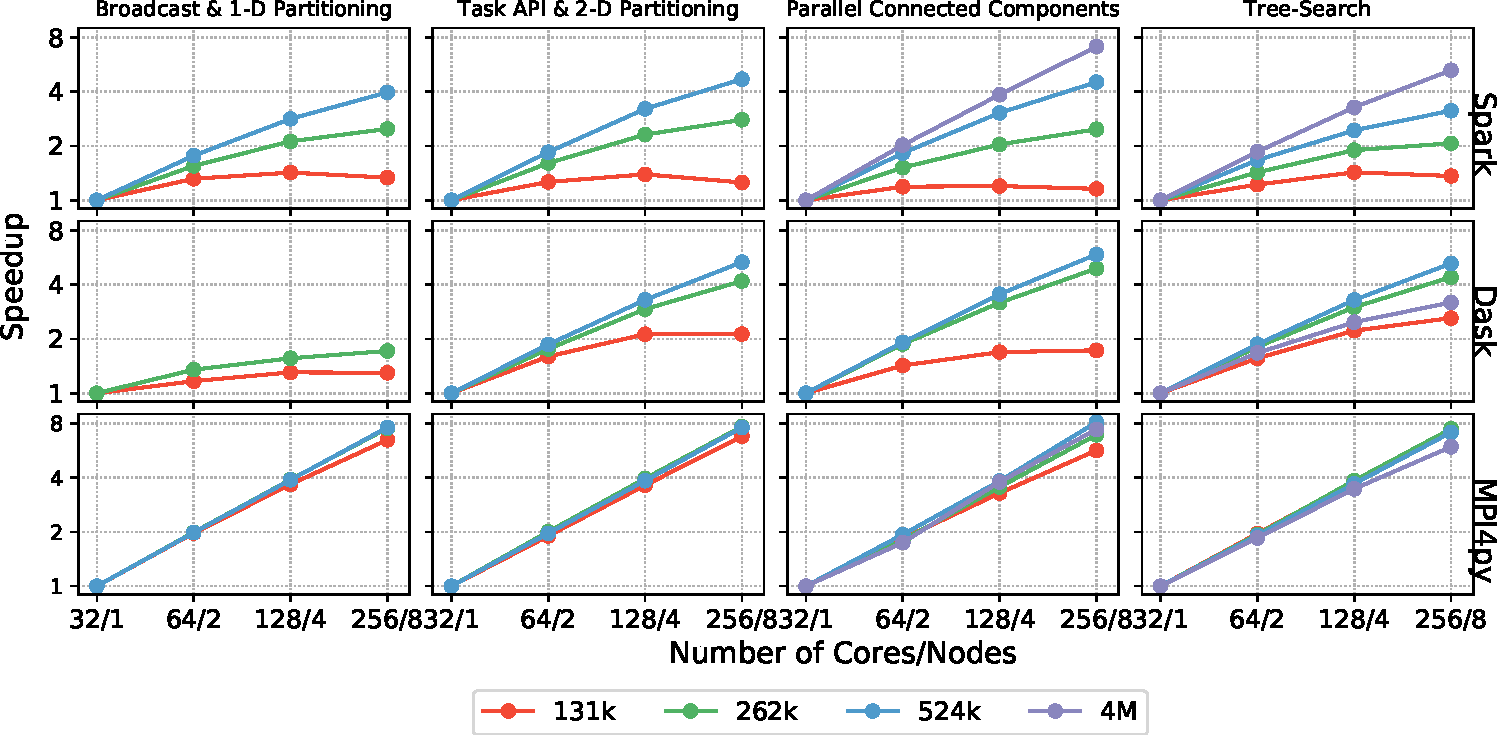
\includegraphics[width=.95\textwidth]{figures/All4approachesWith4MSpeedup.pdf}
    \caption{Selected molecular dynamics analysis MapReduce algorithm speedup 
    for different frameworks and implementation candidates}\label{fig:leafletfinder}
\end{figure*}

The performance analysis of these algorithms implemented in all three frameworks 
provided us with information to create a conceptual model for selecting the 
better suitable framework based on algorithmic characteristics. As shown in 
Figure~\ref{fig:leafletfinder}, there are cases where the performance of a 
parallel implementation is far from ideal, while under different circumstances 
is as expected. Furthermore, non-ideal performance indicates that resource 
utilization is low. For example in Figure~\ref{fig:leafletfinder}, we see that, 
based on data sizem Dask provides better speedup than Spark. In these cases Dask 
better utilized the resources compared to Dask, while on others Spark was 
better.

Implementation aspects, such as computational complexity, and shuffled data 
size influence the performance greatly. For embarrassingly parallel 
applications with coarse grained tasks the choice of the framework does not 
significantly influence performance. For fine-grained data parallelism, a 
data-parallel framework is more suited compared to a workload execution 
framework. In addition, the data shuffling size significantly impacts 
performance and needs to be included in a decision.

Data analysis during scientific campaigns may vary depending on the stage of 
the campaign. As a result, the ability to select the best suited framework, 
given requirements and constraints to execute it is important. This work allows 
us to create that decision making process and include it in the proposed work.
